
\documentclass[12pt,a4paper]{report}
\usepackage[english]{babel}
\usepackage[T1]{fontenc}
\usepackage{times}
\usepackage{amsmath}
\usepackage{amsfonts}
\usepackage{amssymb}
\usepackage{textcomp}
\usepackage{gensymb}
\usepackage{hyperref}
\usepackage{graphicx}
\usepackage{setspace}
\usepackage[version=4]{mhchem}
\usepackage{caption}
\usepackage{subcaption}
\usepackage{longtable}
\usepackage[dvipsnames]{xcolor}
\usepackage{tikz}
\usepackage{wrapfig}
\usepackage[left=2cm,right=2cm,top=2cm,bottom=2cm]{geometry}
\makeatletter
\newcommand\footnoteref[1]{\protected@xdef\@thefnmark{\ref{#1}}\@footnotemark}
\makeatother
\graphicspath{{IMAGE/}}

    \makeatletter
\newcommand{\AlignFootnote}[1]{%
  \ifmeasuring@
  \else
    \iffirstchoice@
      \footnote{#1}%
    \fi
  \fi}
\makeatother



\begin{document}

\begin{titlepage}

\centering

\includegraphics[scale=0.25]{logo_ulg.png}%

\begin{center}\bfseries\huge
\vspace*{1cm}
Modeling and design of electromagnetic systems
\end{center}

\begin{center}\normalsize
Professor: C. Geuzaine\\
\end{center}

\vspace*{\stretch{1}}
\hrulefill
\begin{center}\bfseries\Huge
Homework 3 
\end{center}

\hrulefill
\vspace*{1cm}
\begin{center}\bfseries\Large
Sour Nassim, Heylen Martin
\end{center}

\begin{center}\bfseries\large

Master in electromechanical engineering\\ Bloc 2 \\
University of Liège \\
Academic year: 2019-2020
\end{center}
\vspace*{\stretch{2}}
\begin{flushright}

\end{flushright} 

\end{titlepage}
\setstretch{1.5}
\chapter{Introduction}
\quad\, This project is dedicated to the study of three-phase transformers. Those components are essential in the electrical network to switch from one voltage value to an other, or to reroute some part of the power to equaly distribute the power flow through the different branches of the network. Figure \ref{fig:real_transformer} shows the picture of a typical three-phase transformer.

\begin{figure}[h]
    \centering
    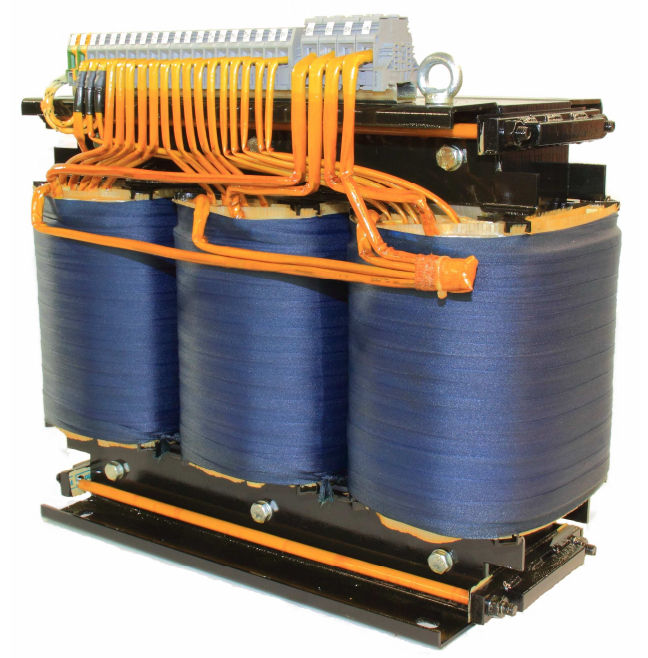
\includegraphics[width=0.4\textwidth]{real_transfo.jpg}
    \caption{Example of real three-phase transformer}
    \label{fig:real_transformer}
\end{figure}
\newpage
\section{Characteristic of the transformers}
Here, the study of two transformers, respectively named \textbf{A} and \textbf{B}) of two different sizes will be considered in this report. The first one is a small transformer that makes the voltage going from 2.4 kV to 240 V for a nominal power of 200 kVA. Defining the transformer ratio $n$ as being the ratio between the high and the low voltage values, For this transformer, the transformer ratio is equal to 
\begin{equation}
    n_A = \frac{2400}{240} = 10
\end{equation}
The second transformer is bigger since it works between the 60 kV and 2.4 kV (leading to a transformer ratio of 25). The nominal power of this transformer is equal to 20,000 KV.

These characteristics supposed that the network is at 50 Hz. Those are summarized in Table \ref{tab:caracteristics_transfo}.

\begin{table}[h]
    \centering
\begin{tabular}{|l|l|l|}
  \hline
   & \textbf{Type A} &\textbf{Type B}\\
  \hline
    Input voltage [V]& 2400 & 60000\\\hline
    Output voltage [V] & 240 & 2400\\\hline
    Output power [kVA] & 200 & 20000\\\hline
    Frequency [Hz] & \multicolumn{2}{c|}{50}\\
  \hline
\end{tabular}
    \caption{Specifications of the two three-phase transformers}
    \label{tab:caracteristics_transfo}
\end{table}

\section{Type of three-phase transformer}
\quad\, When considering a three phase transformer, several configurations regarding to the construction of the core.

The first type of transformer consists in connecting three single-phase transformers together. This configuration is suitable for transformers of large nominal power. Also, "in case of failure of one of the transformers, only that transformer is replaced"\footnote{\url{http://www.montefiore.ulg.ac.be/~vct/elec0014/transp-t.pdf}}. It is also easier to carry.\\

The second type of three-phase transformers are ones for which the core is shared for the three phases. Thus, this implies that the phases are coupled together.

Also, the "volume of this common core is smaller than three times the volume of a single core"\footnote{\url{http://www.montefiore.ulg.ac.be/~vct/elec0014/transp-t.pdf}}.

In this project, the magnetic material used for the core is soft iron for which the saturation induction is around 2T. Also, since it has been said that three individuals core were more suitable for big transformers, transformer \textbf{B} will be design in this way.

\section{Choice of the three-phase transformer connections}
\quad\, Once the core(s) is(are) designed, the second step is to make a decision regarding to the type of connection of the different phases. Basically, considering one side of the transformer, the winding can either be connected in \textcolor{red}{star} or \textcolor{green}{delta}.

The star connection consists in connecting each of three phases to a common nodes which is usually grounded. The star connection is depicted on Figure \ref{fig:star}.
\begin{figure}[h]
    \centering
    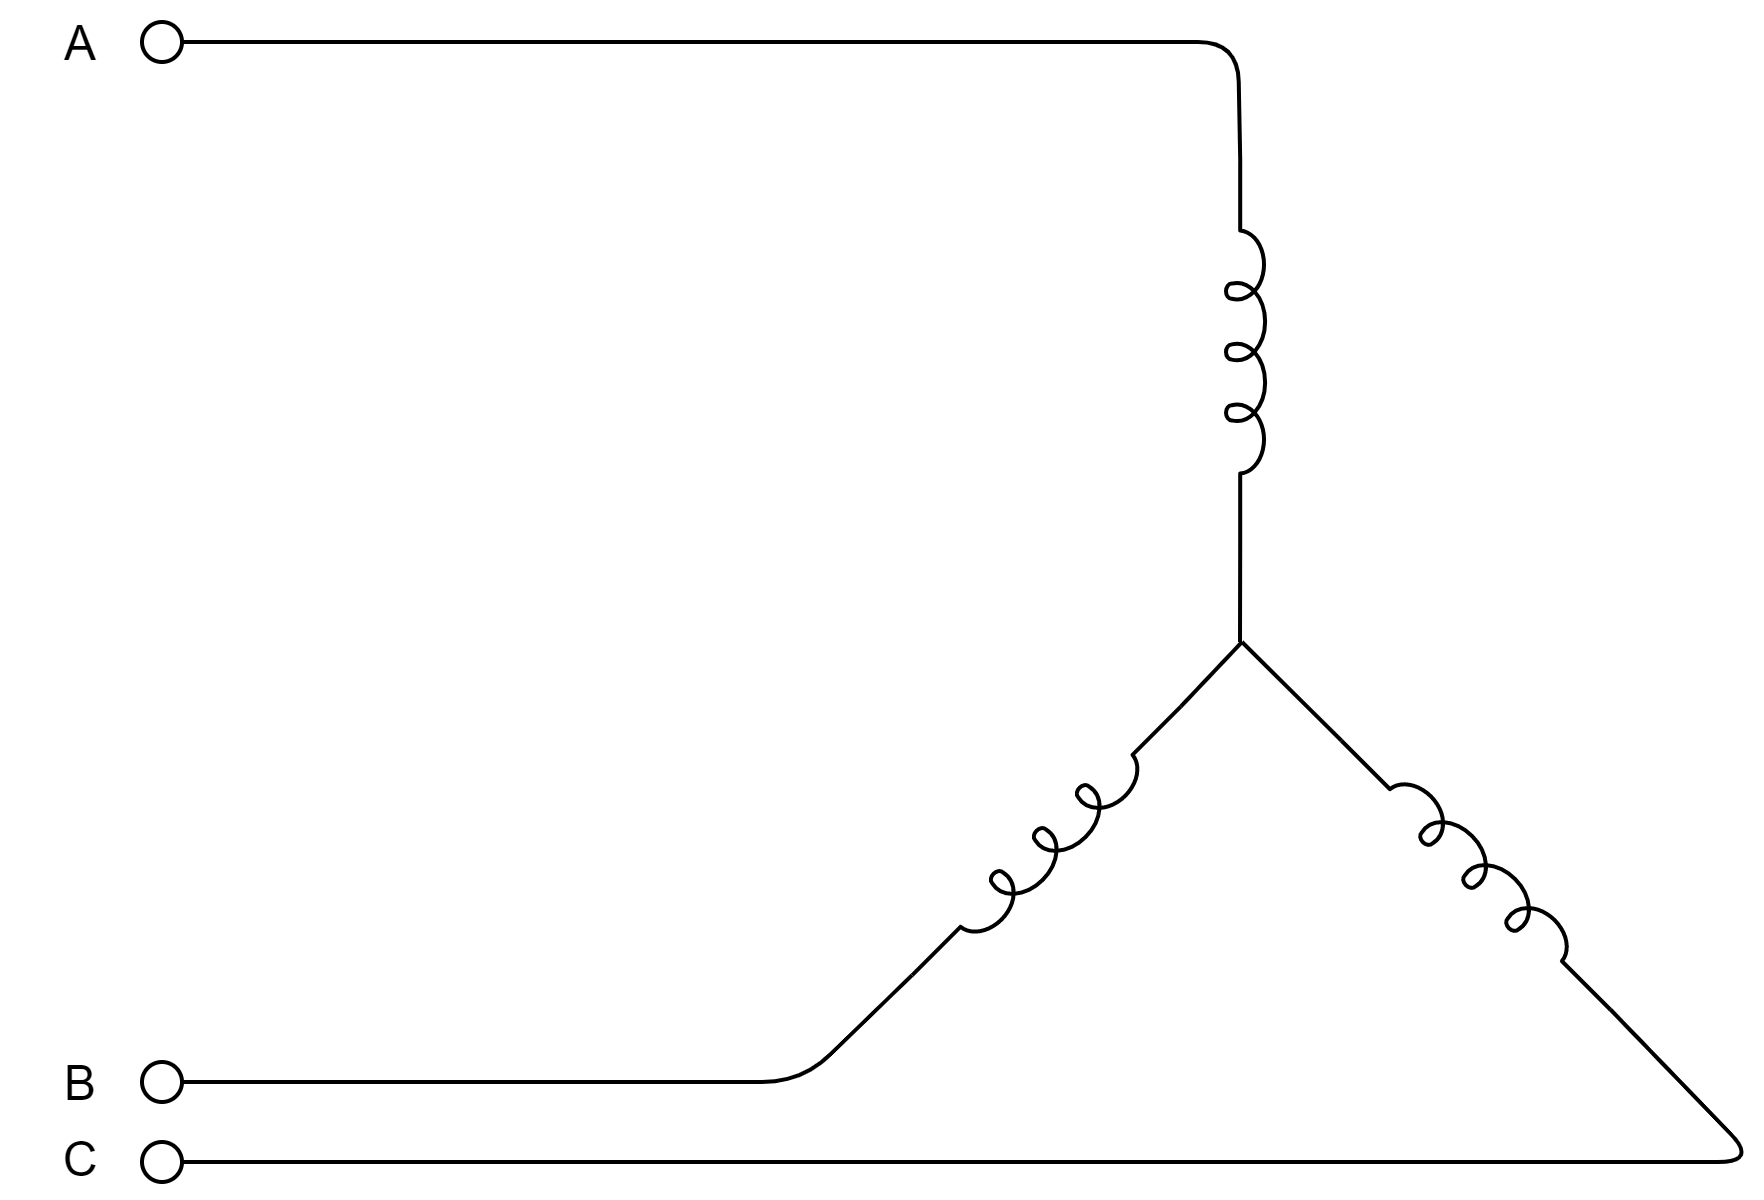
\includegraphics[width=0.6\textwidth]{star.png}
    \caption{Three phase device - Star connection}
    \label{fig:star}
\end{figure}
There are four basic configurations of a three-phase transformer, depending on if the primary or secondary windings are delta- or star-connected. Note that the winding connection options are the same whether using just one three-phase transformer or three separate single phase transformers.
\begin{itemize}
    \item Y-Y :
    
    \begin{figure}[h]
    \centering
    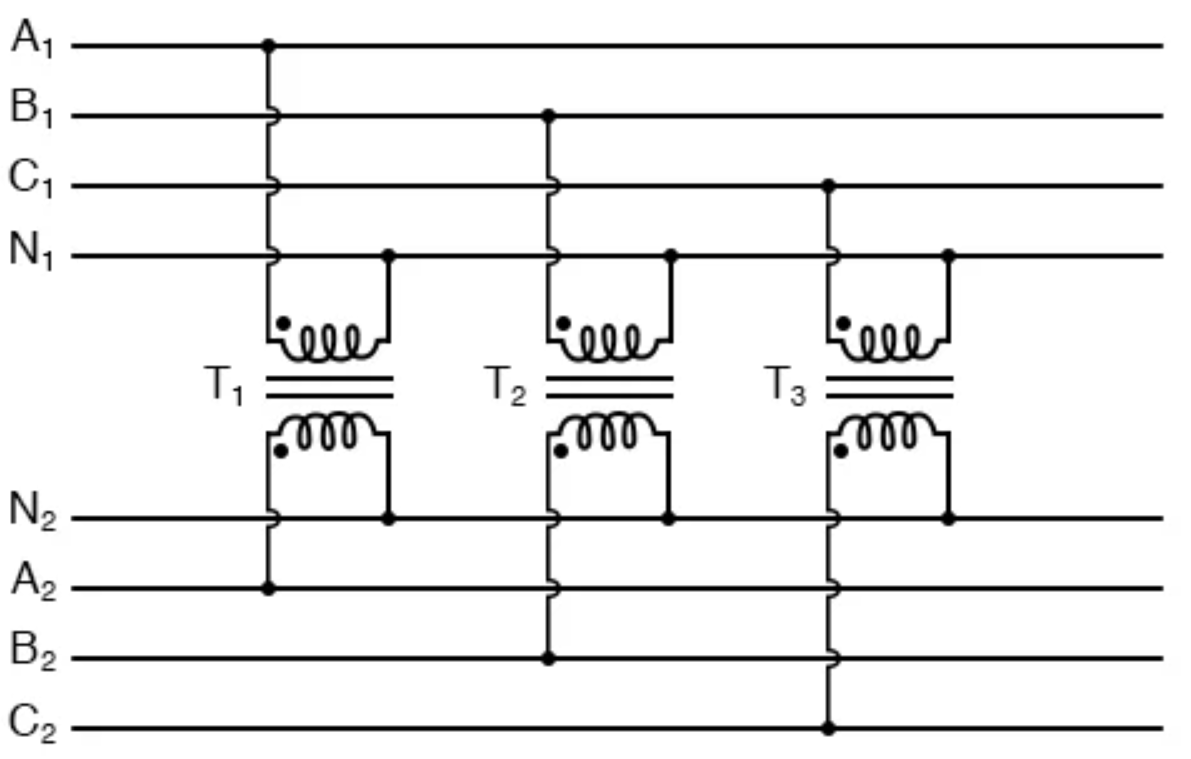
\includegraphics[width=0.6\textwidth]{y-y.PNG}
    \caption{Phase wiring for star-star transformer}
    \label{fig:star-star transformer}
    \end{figure}
    
    \item $\Delta$-$\Delta$ :
       
    \begin{figure}[h]
    \centering
    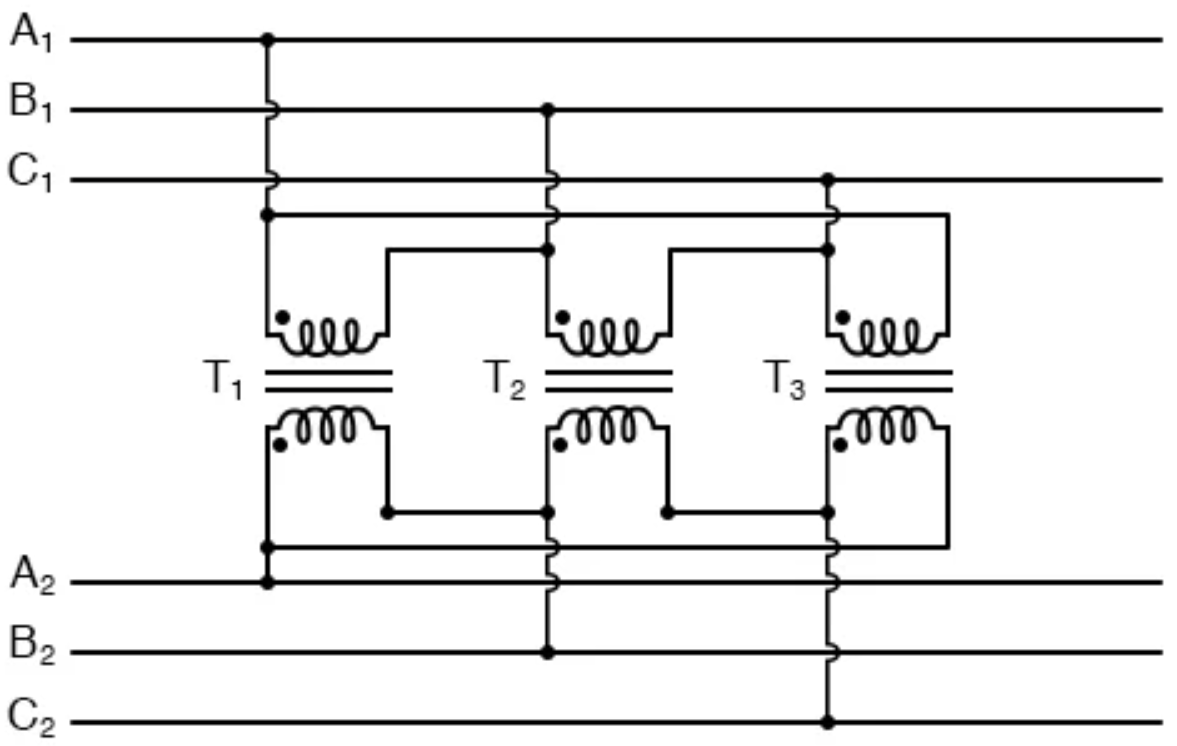
\includegraphics[width=0.6\textwidth]{delta-delta.PNG}
    \caption{Phase wiring for delta-delta transformer}
    \label{fig:delta-delta transformer}
    \end{figure}
    
    \item $\Delta$-Y :
       
    \begin{figure}[h]
    \centering
    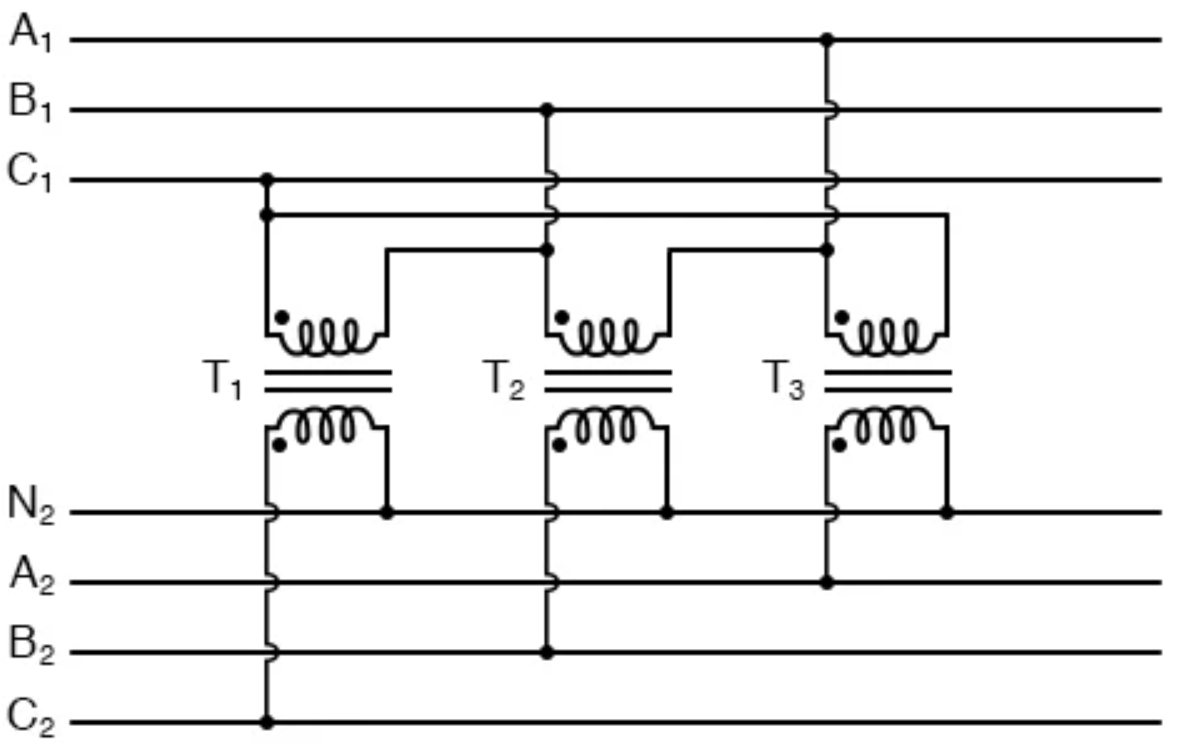
\includegraphics[width=0.6\textwidth]{delta-y.PNG}
    \caption{Phase wiring for delta-star transformer}
    \label{fig:delta-star transformer}
    \end{figure}
    
    \item Y-$\Delta$ :
       
    \begin{figure}[h]
    \centering
    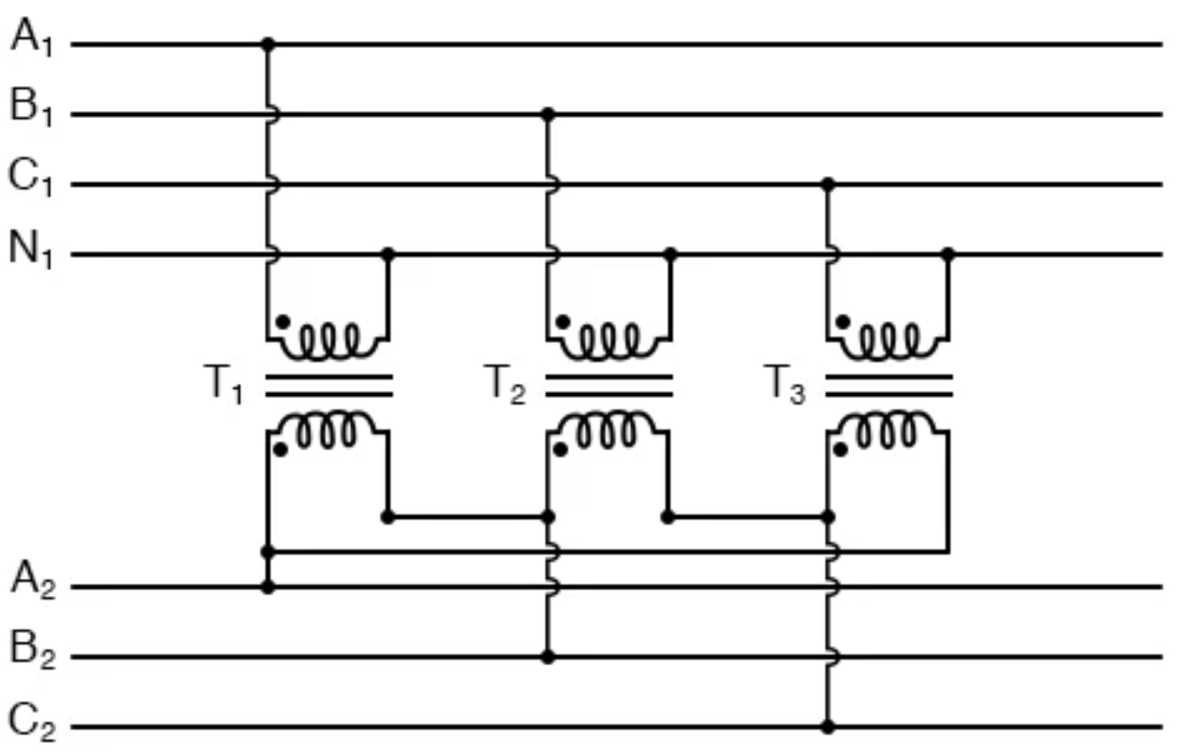
\includegraphics[width=0.6\textwidth]{y-delta.PNG}
    \caption{Phase wiring for star-delta transformer}
    \label{fig:star-delta transformer}
    \end{figure}
\end{itemize}

For this project, $\Delta$-Y connections will be retained. Indeed such a configuration would allow to reduce by a factor $\sqrt{3}$ the current in the phases of the secondary side. Indeed, since the transformer is a step-down transformer, very high current will flow through the secondary.

\section{Calculation of the primary and secondary currents}
After having chosen the primary and secondary connections, primary and secondary currents can be calculated knowing the relations between phase/line voltage and phase/line current. Hence, for the primary currents of the design A :
\begin{equation}
    I_P = \frac{\frac{200000 [VA]}{3}}{2400[V]} = 27,78 [A] = I_L
\end{equation}

For secondary currents of the design A :
\begin{equation}
    I_P = \frac{\frac{200000 [VA]}{3}}{240 [V]} = 277,78 [A]
\end{equation}
and 
\begin{equation}
    I_L = I_P/\sqrt{3} = 160,35[A]
\end{equation}
Analogously, primary and secondary currents for design B have been calculated. Results are shown in Tab. \ref{tab:currents}.

\begin{table}[h]
    \centering
\begin{tabular}{|l|l|l|}
  \hline
   & \textbf{Type A} &\textbf{Type B}\\
  \hline
    Input current [A] & 27,78 & 111,11\\\hline
    Output current [A] & 160,35 & 1603,75\\\hline
\end{tabular}
    \caption{Primary and secondary currents of the two design}
    \label{tab:currents}
\end{table}


%\begin{equation}
%    S_N = \sqrt{3} \cdot V_N \cdot I_N
%\end{equation}
%et avec $S_{1,2}$ et $V_{1,2}$ connus.

\section{Geometry of the windings}
Windings form the electrical circuit of the transformer. Actually, with a too small section, joule losses and heating can be too large. Now that the currents are known, the minimal surface needed for the winding to bear the current can be calculated too. As the maximum current density of the copper is known (J = 2 A/mm$^2$), the following formula can be used :

 \begin{equation}
    I_{1,2} =  J_{Copper} \cdot A_{1,2}
\end{equation}

\begin{table}[h]
    \centering
\begin{tabular}{|l|l|l|l|l|}
  \hline
    & \multicolumn{2}{c|}{\textbf{Type A}} & \multicolumn{2}{c|}{\textbf{Type B}}\\\hline
    Currents [A] & 27,78 & 160,35 & 111,11 & 1603,75\\\hline
    Area [mm$^2$] & 13,89 & 80,175 & 55,55 & 801,875\\\hline
    Radius [mm] & 2,1 & 5,1 & 4,2 & 16\\\hline
\end{tabular}
    \caption{Minimum area of the coils}
    \label{tab:windings_area}
\end{table}

Basically there are different types of winding (cylindrical, helical, continuous disc,...) according to the transformer ratings (kVA). For the sake of simplification, only cylindrical and circular conductors will be considered here.

\section{Calculation of the number of turns}
Let's define the transformers turns ratio as :
\begin{equation}
     N =  \frac{N_2}{N_1}
\end{equation}
which is equal, for an ideal transformer, to :
\begin{equation}
\frac{N_2}{N_1} = \frac{V_2}{V_1}
\end{equation}
That leads to turns ratio values of $N_A = 25$ for the first type and $N_B = 10$ for the second one.\\

We can compute the conditions on the number of turns to not exceed the saturation induction of the chosen magnetic material, which is the soft iron. Using Faraday's Law, we have :

\begin{equation}
    V_1 = N_1 \cdot \mid \frac{d\phi(t)}{dt} \mid = N_1 \cdot \frac{d(B(t)\cdot S)}{dt} = N_1 \cdot \omega \cdot B \cdot S
\end{equation}
where \textit{S} is the cross-section area of the core \textcolor{red}{ajouter aire du core} and $\omega$ is the pulsation at 50 Hz. Knowing that the maximum magnetic flux density for soft iron is around 2 tesla, the following condition has to be respected :
\begin{equation}
    B < B_{max} = 2 [T]
\end{equation}
Therefore, 
\begin{equation}
       \frac{V_1}{N_1 \cdot \omega \cdot S} < 2
\end{equation}
Hence,
\begin{equation}
N_1 > \frac{V_1}{\omega \cdot 2 \cdot S}
\end{equation}

Finally, the condition on the number of turns on the secondary coil is computed using the transformers turns ratio and we have $N_2 < ...$.

 \textcolor{red}{Rajouter qualité du bobinage}\\
 \textcolor{red}{Déterminer S pour chaque phase et donc $N_1$ et $N_2$ pour chaque phase}\\
\textcolor{red}{Ajouter la charge de 1000 $\ohm$ pour vérifier la capacité du transfo}

\section{Selection for core design}
\subsection{Comparison of core- and shell-type designs}
The most difference that exists between core- and shell-type design is that in core-type design the winding encircles the core as they are placed on two core limb and for shell-type design the core encircles most of the part of the windings as they are placed on mid arm of the core. That leads to single magnetic circuit in core-type while there are two magnetic flux paths for shell-type, as can be seen from Fig. \ref{fig:shell_core_type}.

 \begin{figure}[h]
    \centering
    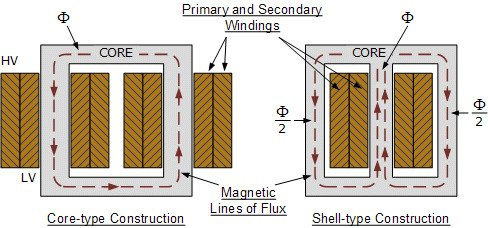
\includegraphics[width=0.6\textwidth]{type_design_2.jpg}
    \caption{Types of three-phase transformers design}
    \label{fig:shell_core_type}
\end{figure}


\subsection{Geometry of the design}
These designs have been performed using \textit{gmsh} and are shown in the Fig.\\
\textcolor{red}{+ ajouter les deux geos}

\begin{table}[h]
    \centering
\begin{tabular}{|l|l|l|l|l|}
  \hline
   & \multicolumn{2}{c|}{\textbf{Type A}} & \multicolumn{2}{c|}{\textbf{Type B}}\\\hline
   \textbf{Type design} & \textbf{Shell} & \textbf{Core} & \textbf{Shell} & \textbf{Core}\\\hline
   $N_1$ [turns]& & & &\\\hline
    $N_2$ [turns]& & & &\\\hline
    Width of the core [cm]& & & &\\\hline
    Thickness of the core [cm]& & & &\\\hline
    Total height of the transformer [cm]& & & &\\\hline
    Total width of the transformer [cm]& & & &\\
  \hline
\end{tabular}
    \caption{Geometry of the two three-phase transformers}
    \label{tab:designed_transfo}
\end{table}

+ Calculer les rendements des deux transfos :

\begin{equation}
   \eta = \frac{P_2}{P_1}
\end{equation}

\section{Transformer tests}

\subsection{Equivalent circuit}
There are two kind of tests : open and short circuit tests. They are both performed to determine the equivalent circuit of transformer, its voltage regulation and efficiency.
The power required for these tests is equal to the power loss occurring in the transformer.

 \begin{figure}[h]
    \centering
    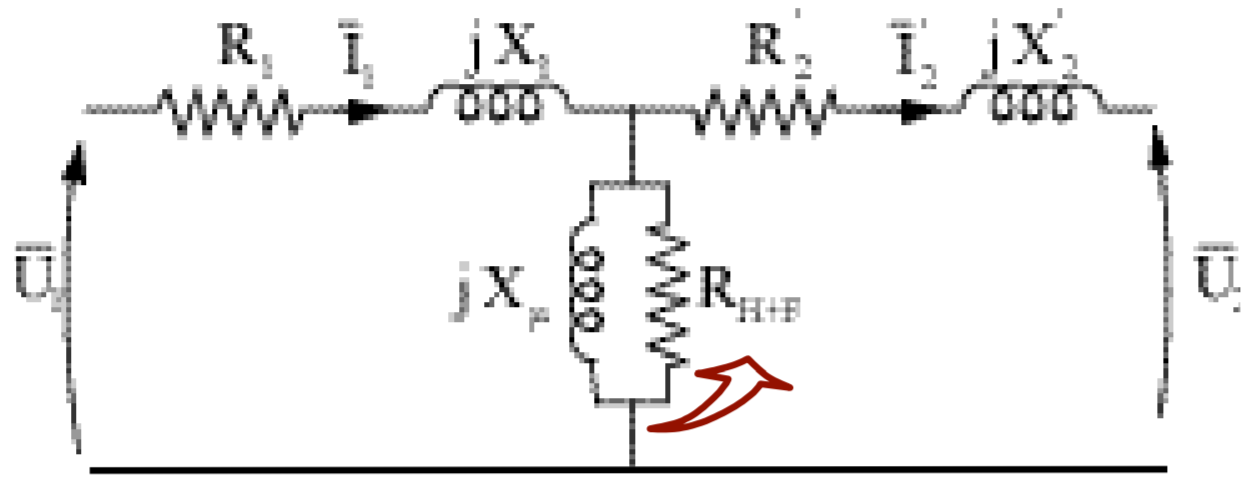
\includegraphics[width=0.6\textwidth]{equivalent_circuit.PNG}
    \caption{Transformer equivalent circuit}
    \label{fig:equivalent_circuit}
\end{figure}

\subsubsection{Open-load test}
Calculate the core loss Calcul des pertes dans le circuit magnétique  $R_{H,F}$ et $X_\mu$ :

\begin{equation}
   P_V = \frac{U_1^2}{R_{H,F}}
\end{equation}
\begin{equation}
   Q_v = \frac{U_1^2}{X_{\mu}}
\end{equation}

\subsubsection{Short-circuit test}
Calculate the total copper loss in the windings ,Calcul des résistances électriques des deux côtés + réactance de fuite :
\begin{equation}
P_{cc} = (R_1 + R_2') \cdot I_{cc}^2
\end{equation}
\begin{equation}
Q_{cc} = (X_1 + X_2') \cdot I_{cc}^2
\end{equation}

+ Tableau récapitulatif des valeurs

\subsubsection{Exterior characteristic}
Tracer le graphe caractéristique U-I pour chaque transfo

\section{Additional parametric studies}

\subsection{Effect of the winding electric resistivity}
Tracer le graphe de $\eta$ en fonction de $\rho$
\subsection{Effect of the core magnetic permeability}
Par exemple, tracer le graphe de $\eta$ en fonction de $\mu$
\subsection{Effect of the presence of an air gap}
Un air gap apporte une réluctance en série tel que :

\begin{equation}
    R_{fer} << R_{air}
\end{equation}
Vu que 
\begin{equation}
   R = \frac{1}{\mu} \cdot \frac{d}{S}
\end{equation}
et
\begin{equation}
   \mu_{fer} >> \mu_{air}
\end{equation}
Tracer le graphe de $\eta$ en fonction de l'air gap (< 0,1 mm)

\subsection{Effect of a non-laminated core}
Etant donné que le but du fer lamellé c'est diminuer les pertes par effet joule dûs aux courants de Foucault, on peut essayer de simuler du fer lamellé en faisant diminuer progressivement la conductivité électrique du noyau et voir l'impact sur le rendement $\eta$
--> graphe de $\eta$ en fonction de la conductivité $\sigma$
\subsection{Effect of shielding the transformer}
Shielding the transformer consists in surrounding it with a tank. +blabla\\

En pratique, rajouter une volume qui englobe le transfo dans la géométrie. Normalement, un bouclier n'augmente pas des masses le rendement du transfo.

\subsection{Effect of higher operating frequencies}
Calcul de la gamme de fréquence dans laquelle le transfo est censé fonctionner [$f_{min}$,$f_{max}$] + Que se passe-t-il si on augmente les 50 Hz ?\\

Par exemple, tracer le graphe de $\eta$ en fonction de $f$ ou $\omega$

\subsection{Effect of the loss of one phase}
%The effect of the loss of one phase also depends on the reasons for choosing a star or delta configuration for transformer winding connections. For example, star connections allows high range of voltages while delta connections are more reliable, meaning that if one winding stop working the other two can still maintain full line voltages to the load.

\section{Conclusion - Limitations - Further work}
Mettre les limites du modèle (cooling methods, insulating oil not discussed here, sélection du type d'enroulement selon la puissance apparente, ..)

\end{document}
